\documentclass[12pt, runningheads,a4paper]{llncs}
%

\usepackage{natbib} % bibliography stuff
%
\usepackage{graphicx} % allows for working with images
\DeclareGraphicsExtensions{.pdf,.png,.jpeg} % configures latex to look for the following image extensions
%
\usepackage{setspace} % allows for configuring the linespacing in the document
%\singlespacing
\onehalfspacing
%\doublespacing
%
\usepackage{amsmath}
%
\usepackage{appendix}
%
\usepackage{fancyvrb}
%
\usepackage{multirow}
%
\usepackage{booktabs,array,dcolumn}
%
\usepackage{eurosym}
%
\usepackage{listings}
\usepackage{caption}
\captionsetup[table]{skip=10pt}
\captionsetup{compatibility=false}
\usepackage{subcaption}
%
\usepackage[toc]{glossaries}
\makeglossaries

\usepackage{glossaries}

\newglossaryentry{sample}{name={sample},description={an example}}

\renewcommand{\glstextformat}[1]{\textit{#1}}

%
\usepackage{amssymb}
\setcounter{tocdepth}{4}
%
\usepackage{url}
\urldef{\mailsa}\path|20064376@mail.wit.ie|
\newcommand{\keywords}[1]{\par\addvspace\baselineskip
\noindent\keywordname\enspace\ignorespaces#1}

%Optional Package to add PDF bookmarks and hypertext links
\usepackage[pdftex,hypertexnames=false,linktocpage=true]{hyperref}
\hypersetup{colorlinks=true,linkcolor=black,anchorcolor=black,citecolor=black,filecolor=black,urlcolor=black,bookmarksnumbered=true,pdfview=FitB}
\usepackage[dvipsnames,cmyk]{xcolor}

% --------------------------------------------------------------
% Colors
% --------------------------------------------------------------
\definecolor{editorGray}{cmyk}{0, 0, 0, 0.2}
\definecolor{editorBlue}{cmyk}{1, 0.35, 0, 0}
\definecolor{editorPink}{cmyk}{0, 1, 0, 0}
\definecolor{editorDarkOrange}{cmyk}{0, 0.8, 0.9, 0}
\definecolor{editorGray}{gray}{0}
\definecolor{editorPurple}{cmyk}{0.75, 1, 0, 0}
% ----------------------------------------------------------------------
%  CSS
% ----------------------------------------------------------------------
\newcommand{\CodeSymbol}[1]{\textcolor{editorPink}{#1}}

\lstdefinelanguage{CSS3}{
  sensitive=true,
  tagstyle=\color{editorBlue},
  markfirstintag=true,
  % Line numbers
  xleftmargin={20pt},
  numbers=left,
  stepnumber=1,
  firstnumber=1,
  numberfirstline=true,
  numberstyle=\color{black},
  frame=l,
  % Keywords
  ndkeywords={accelerator,azimuth,background,background-attachment,
        background-color,background-image,background-position,
        background-position-x,background-position-y,background-repeat,
        behavior,border,border-bottom,border-bottom-color,
        border-bottom-style,border-bottom-width,border-collapse,
        border-color,border-left,border-left-color,border-left-style,
        border-left-width,border-right,border-right-color,
        border-right-style,border-right-width,border-spacing,
        border-style,border-top,border-top-color,border-top-style,
        border-top-width,border-width,bottom,caption-side,clear,
        clip,color,content,counter-increment,counter-reset,cue,
        cue-after,cue-before,cursor,direction,display,elevation,
        empty-cells,filter,float,font,font-family,font-size,
        font-size-adjust,font-stretch,font-style,font-variant,
        font-weight,height,ime-mode,include-source,
        layer-background-color,layer-background-image,layout-flow,
        layout-grid,layout-grid-char,layout-grid-char-spacing,
        layout-grid-line,layout-grid-mode,layout-grid-type,left,
        letter-spacing,line-break,line-height,list-style,
        list-style-image,list-style-position,list-style-type,margin,
        margin-bottom,margin-left,margin-right,margin-top,
        marker-offset,marks,max-height,max-width,min-height,
        min-width,-moz-binding,-moz-border-radius,
        -moz-border-radius-topleft,-moz-border-radius-topright,
        -moz-border-radius-bottomright,-moz-border-radius-bottomleft,
        -moz-border-top-colors,-moz-border-right-colors,
        -moz-border-bottom-colors,-moz-border-left-colors,-moz-opacity,
        -moz-outline,-moz-outline-color,-moz-outline-style,
        -moz-outline-width,-moz-user-focus,-moz-user-input,
        -moz-user-modify,-moz-user-select,orphans,outline,
        outline-color,outline-style,outline-width,overflow,
        overflow-X,overflow-Y,padding,padding-bottom,padding-left,
        padding-right,padding-top,page,page-break-after,
        page-break-before,page-break-inside,pause,pause-after,
        pause-before,pitch,pitch-range,play-during,position,quotes,
        -replace,richness,right,ruby-align,ruby-overhang,
        ruby-position,-set-link-source,size,speak,speak-header,
        speak-numeral,speak-punctuation,speech-rate,stress,
        scrollbar-arrow-color,scrollbar-base-color,
        scrollbar-dark-shadow-color,scrollbar-face-color,
        scrollbar-highlight-color,scrollbar-shadow-color,
        scrollbar-3d-light-color,scrollbar-track-color,table-layout,
        text-align,text-align-last,text-decoration,text-indent,
        text-justify,text-overflow,text-shadow,text-transform,
        text-autospace,text-kashida-space,text-underline-position,top,
        unicode-bidi,-use-link-source,vertical-align,visibility,
        voice-family,volume,white-space,widows,width,word-break,
        word-spacing,word-wrap,writing-mode,z-index,zoom},
  morecomment=[l][\color{darkgray}]{//},
  morecomment=[s][\color{darkgray}]{/*}{*/},
  morestring=[s]{:}{;}, 
  alsoletter={.\#{}},
  alsodigit={-},
  literate={\{}{{\CodeSymbol{\{}}}1
           {\}}{{\CodeSymbol{\}}}}1
           {>}{{\CodeSymbol{>}}}1
}
% ----------------------------------------------------------------------
%  HTML
% ----------------------------------------------------------------------
\lstdefinelanguage{HTML5}{
  language=html,
  sensitive=true,
  tagstyle=\color{editorBlue},
  markfirstintag=true,
  morecomment=[s][\color{darkgray}]{<!-}{-->},
  alsoletter={!-'},
  keywords={},
  % Line numbers
  xleftmargin={14pt},
  numbers=left,
  stepnumber=1,
  firstnumber=1,
  numberfirstline=true,
  numberstyle=\color{black},
  % Frame
  frame=l,
}
% ----------------------------------------------------------------------
%  Code style
% ----------------------------------------------------------------------
\lstset{%
  % General design
  inputencoding=utf8,
  backgroundcolor=\color{white},
  basicstyle=\normalsize\ttfamily\upshape\lst@ifdisplaystyle\scriptsize\fi,
  frame=none,
  escapeinside=`',
  % Code design
  stringstyle=\color{editorPurple},
  commentstyle=\color{editorGray},
  keywordstyle=\color{editorPink},
  ndkeywordstyle=\color{editorBlue},
  identifierstyle=\color{editorDarkOrange},
  commentstyle=\color{editorGray},
  % Languages
  language=HTML5,
  alsolanguage=CSS3,
  % Code
  alsodigit={.:},
  tabsize=2,
  showtabs=false,
  showspaces=false,
  showstringspaces=false,
  extendedchars=true,
  breaklines=false,
}

\begin{document}
\mainmatter  % start of an individual contribution

% first the title is needed
\title{Final Project Report (Taylor'd UI)}

% a short form should be given in case it is too long for the running head
\titlerunning{Semester Two Project Report}

% the name(s) of the author(s) follow(s) next
%
% NB: Chinese authors should write their first names(s) in front of
% their surnames. This ensures that the names appear correctly in
% the running heads and the author index.
%
\author{Michael Taylor,%
%\thanks{Please note that the LNCS Editorial assumes that all authors have used
%the western naming convention, with given names preceding surnames. This determines
%the structure of the names in the running heads and the author index.}%
\and Eamonn De'Leaster\thanks{Supervisor}}
%
\authorrunning{Michael Taylor 20064376}
% (feature abused for this document to repeat the title also on left hand pages)

% the affiliations are given next; don't give your e-mail address
% unless you accept that it will be published
\institute{Waterford Institute of Technology,\\Dept of Computing and Mathematics,\\
Cork Rd, Waterford City, Ireland\\
\mailsa\\
\url{http://www.wit.ie}}

%
% NB: a more complex sample for affiliations and the mapping to the
% corresponding authors can be found in the file "llncs.dem"
% (search for the string "\mainmatter" where a contribution starts).
% "llncs.dem" accompanies the document class "llncs.cls".
%
%\toctitle{Thesis Proposal}
\tocauthor{M. Taylor}
\maketitle

%
\begin{abstract}

A complete User Interface framework designed for entry level users with a focus on a vocabulary that is easy to understand. Taylor'd UI will also introduce partials using web components, boilerplate code offering different themes and integrated command line interface.
\keywords{CSS, User Interface, framework, beginners, boilerplate, partials, themes}
\end{abstract}
%

%
%\newpage
%\chapter*{Acknowledgements}

This dissertation would not have been possible without the support of the following people.

To my supervisors Alan and John for their patience, guidance and sharing of knowledge during this process. Thank you, it has been a real pleasure working together.

To my lecturers at the Waterford Institute of Technology, you have all been so open and free with your sharing of knowledge, it has been an absolute pleasure learning from you.

To my partner Michael, I'm keenly aware standing in the freezing cold at 02:00 helping me put up radio antennas might not have been the most exciting thing you've partaken in all year, but I couldn't have done it without your help. Thanks for your constant encouragement and for putting up with me during this. 

To my sister Jean, you inspired me to work as hard as I have these last 6 years. I wanted to make you as proud of me as I am of you. If you beat me to Ph.D, I'll buy you a bag of chips in Roccos.

To my father, I can only imagine the conversations we might have had, I suspect you would have loved playing with this equipment as much as I have.

To my mother, thank you for your friendship. You have always been a positive influence in my life. Some day you must sit down and explain how you can walk past, and in the time it takes to cross a room and without any prior involvement, solve a problem I have been struggling with for days.

To my four dogs Noah, Oscar, Rosie and Dora, you are the best mutts a man could ask for.
%
\newpage
\tableofcontents
%
\renewcommand*{\glsclearpage}{}
\printglossaries
%%
\newpage
\listoffigures
\addcontentsline{toc}{chapter}{List of Figures}
\listoftables
\addcontentsline{toc}{chapter}{List of Tables}
%%%%%%%%%%%%%%%%%%%%%%%%%%%%%%%%%%%%%%%%%%%%%%%%%%%%%%%%%%%%%%%%%%%%%%%%%%%%%%%%%%%%%%
%%

%
\chapter*{Acknowledgements}

This dissertation would not have been possible without the support of the following people.

To my supervisors Alan and John for their patience, guidance and sharing of knowledge during this process. Thank you, it has been a real pleasure working together.

To my lecturers at the Waterford Institute of Technology, you have all been so open and free with your sharing of knowledge, it has been an absolute pleasure learning from you.

To my partner Michael, I'm keenly aware standing in the freezing cold at 02:00 helping me put up radio antennas might not have been the most exciting thing you've partaken in all year, but I couldn't have done it without your help. Thanks for your constant encouragement and for putting up with me during this. 

To my sister Jean, you inspired me to work as hard as I have these last 6 years. I wanted to make you as proud of me as I am of you. If you beat me to Ph.D, I'll buy you a bag of chips in Roccos.

To my father, I can only imagine the conversations we might have had, I suspect you would have loved playing with this equipment as much as I have.

To my mother, thank you for your friendship. You have always been a positive influence in my life. Some day you must sit down and explain how you can walk past, and in the time it takes to cross a room and without any prior involvement, solve a problem I have been struggling with for days.

To my four dogs Noah, Oscar, Rosie and Dora, you are the best mutts a man could ask for.
\newpage
\chapter*{Introduction}
\addcontentsline{toc}{chapter}{Introduction}
\section*{Background}
\addcontentsline{toc}{section}{Background}

\gls{UI}, and \gls{CSS} frameworks are abundant and readily available and generally covered by permissible licence agreements \citep{CODY16}. This not only allows commercial use of the frameworks but ultimately encourages tie in to a particular framework. End users expect all websites to work across their devices, laptops, tablets and phones. This requirement of responsive web applications ensures that hand coding a solution is a daunting task for entry level developers.

%
\newglossaryentry{CSS}
{
  name={CSS},
  description={Cascading Stylesheets},
  sort=CSS
}
%


%
\newglossaryentry{UI}
{
  name={UI},
  description={User Interface},
  sort=UI
}
%

\newglossaryentry{HTML}
{
  name={HTML},
  description={HyperText Markup Language},
  sort=HTML
}

Using a framework allows the user to speed up the initial mock-up process, they offer clarification on common \gls{CSS} issues, and have wide browser support. Frameworks are good for responsive design, offer clean, and tidy code. There are disadvantages to using frameworks such as an abundance of unused code left over, this is seen more so in large front end frameworks such as Twitter Bootstrap. There is a slower learning curve with using frameworks, as the majority of work is done for them, users tend to make only minor changes such as modifications to colour.

Frameworks such as Twitter Bootstrap \citep*{SASS16}, and Zurb Foundation \citep*{LESS16} offer complete solutions, with ready built code for forms, buttons, fluid layouts, and popovers. Skeleton is an example of the other end of the spectrum. Skeleton is a boilerplate for responsive, and mobile first development. It is designed to be light, and is built with less than 400 lines of code \citep{SKEL16}. Unlike Bootstrap or Foundation, Skeleton is designed to be the users starting point, not their full solution. 

Taylor'd UI has been designed and built with the intension of offering a complete solution aimed at an entry level user. The framework is non-opinionated unlike frameworks such as Bootstrap which is very opinionated about their design \citep{KEMH16}. This framework is designed to be the starting point which a user may then manipulate, and build upon.

Rather than building large complex websites with repeating code, one of the project goals is to allow a safe environment where a user can experiment with templates, partials. Partials break up the \gls{HTML} code into smaller more manageable fragments that can be used across multiple \gls{HTML} files. The framework has been built with this in mind, creating classes, and id's that can be reused instead of having a bloated package with a lot of unused code \citep{KAR15}.

\newglossaryentry{CLI}
{
  name={CLI},
  description={Command Line Interface},
  sort=CLI
}

Prebuilt code such as standard default themes are often referred to as a template. A major benefit of this project is to enable the easy modification of such templates. By generating the templates for the user, it can allow them to concentrate on the aesthetics more so than the structure of the project. Using prebuilt themes will not suit every situation. The templates themselves can be expensive as can be seen on Themeforest \citep{THEME17}, and might not adhere to the W3C standards, or worse might offer little customisation \citep{NATH16}. 

Further attempts to incorporate Bootstrap into projects demonstrated the syntax as very unfriendly, and noticeably more difficult than hand coded \gls{CSS}. Bootstrap syntax such as: \begin{lstlisting}
	 <div class="col-sm-4">\end{lstlisting} 
	 does not describe in any form that it would be displayed as a three column layout in the browser. Based on the snippet above, an entry level user is unlikely to know how to change this from a three column layout to a single column layout. 
	 
Additionally while working as a web developer mentor at Coderdojo, students were observed to have similar experiences. Many were reluctant to learn frameworks such as Bootstrap as they were too confusing. Taylor'd UI could potentially be used in an educational environment to provide students a structured introduction to web development.

The framework will contain similar features from both Bootstrap, and Foundation as seen in table \ref{features} such as tables, lists, breadcrumbs, and pagination. Features such as tooltips, and right to left language support are outside the scope of the project. The hope for the project is to be complete framework but having a smaller file size than both foundation, and Bootstrap borrowing concepts from Skeleton in keeping the framework light, and nimble. Taylor'd UI has five major aspects to it: 
\begin{itemize}
	\item For entry level users
	\item Theme-able
	\item Introduce the concepts of partials
	\item Have templates for the user to manipulate
	\item Install framework from the command line
\end{itemize}
%
\newpage
\section*{License}
\addcontentsline{toc}{section}{License}
The application will be released under the MIT license following in the footsteps of the other frameworks researched for this project. The MIT license is permissive, allowing permissions such as commercial use, private use, distribution, and modification. With the MIT license, another user cannot claim the work as their own, derivatives are allowed as long as the original author is credited, and the original authors cannot be held liable.

The link to this project can be found at:

https://github.com/MikeZTaylor/Taylord-UI

\newpage
\chapter*{User Manual}
\addcontentsline{toc}{chapter}{User Manual}
\section*{Introduction}
\addcontentsline{toc}{section}{Introduction}
% Chapter for each research question
% how we validated it and proved it worked

The project is to build a full \gls{UI} framework that is aimed towards an entry level user. The framework is be non-opinionated, light weight, easy to understand, theme-able, and most importantly easy to learn.

The framework has minimal styling, the author has only added styling where it is needed, and that styling is kept to basic colours. This was to ensure the framework does not carry the author's design opinions. With been non-opinionated the framework is bare so that the end user is encouraged to not rely upon the built in styling, but instead to use it as a starting point to build upon it. The framework is based on a responsive grid system of 12 grids, allowing the end user to build a seamless experience from desktops to mobile devices.

The hope is that the framework will be as small of possible as of the source code deadline, the framework weighs ----- this allows projects using it load faster on mobile devices, and in countries where fast internet is either not available or expensive. 

To stop code from been repeated unnecessary, code sections have been broken into partials allow for the ability for the content to be broken up into manageable pieces, removing receptive code such as headers, and footers. PHP is then used to combine the files into one when loaded in the browser. 

\newpage
The framework will contain similar features from both Bootstrap, and Foundation as seen in table \ref{features} such as tables, lists, breadcrumbs, and pagination. Features such a tooltips, and right to left are outside the scope of the project. The hope for the project is to be complete framework but having a smaller file size than both foundation, and Bootstrap borrowing concepts from Skeleton in keeping the framework light, and nimble. 

The proposed framework will be built using the three key points mentioned below: 
\begin{itemize}
	\item For Entry Level Users
	\item Themeable
	\item Introduce the concepts of Templates, and Partials
\end{itemize}

\newpage
\chapter*{Partials}
\addcontentsline{toc}{chapter}{2. Partials}
% Chapter for each research question
% how we validated it and proved it worked


Partials are reusable \gls{HTML} snippets that you can be embed into a template file and render, this helps you modularise your development. By splitting up the code into partials, you are:

\begin{itemize}
	\item Keeping your code clean and systematic
	\item Adhering to the \gls{DRY} philosophy
	\item Creating reusability
	\item Aid in fragment caching
\end{itemize}

Not all modern browsers have full support for partials, and templates as seen on the website caniuse \citep*{CANI17}. In order to achieve partials, and templates, Taylor'd UI is using nunjucks a rich and powerful templating engine. 

If you are not comfortable in learning how to break the \gls{HTML} into partials, and just want the \gls{HTML} file to play around with, the file \latinword{index.html} can be found in the parent directory.

Before starting, from the terminal enter in the commands seen below, the first will install gulp, the second will install nunjucks:

\begin{lstlisting}[language=HTML]
npm install gulp-cli -g
npm install gulp-nunjucks-render --save-dev
\end{lstlisting}

A package.json file will then need to be created, this will configure the Node / NPM packages. Following this, create a \latinword{gulp.js} file, and place it in your main folder. Open the file and add the two following lines to the top.:

\begin{lstlisting}[language=HTML]
var gulp = require('gulp');
var nunjucksRender = require('gulp-nunjucks-render');
\end{lstlisting}

The \latinword{gulp.js} file tells gulp what to do. In this file, we will be adding in the tasks we want gulp to run.

Next, create a folder structure similar to layout structure as seen in figure \ref{fig:structure}. The templates folder is used for storing the Nunjucks partials, and any other Nunjucks files that will be added to files in the pages folder. The pages folder is used for storing files that will be compiled into \gls{HTML}. Once they are compiled, they will be created in the blog folder.

Create a file and call it \latinword{layout.nunjucks}. The layout file will contain the template \gls{HTML} code such as title, and links to external files such as the\gls{CSS}.
{
  name={CSS},
  description={Cascading Stylesheets},
  sort=CSS
}, see below for an example.

\begin{lstlisting}[language=HTML]
<!-- layout.nunjucks -->
<!DOCTYPE html>
<html lang="en">
<head>
  <meta charset="UTF-8">
  <title>Simple Blog</title>
  <link rel="stylesheet" href="css/taylord.css" />
</head>
<body>

  <!-- You write code for this content block in another file -->
   
</body>
</html>
\end{lstlisting}

In the pages folder, create a file called \latinword{index.nunjucks}. This file will ultimately be converted into index.html and placed in the blog folder. The \latinword{index.nunjucks} extends the \latinword{layout.nunjucks} file, this means it contains all the template code written in the layout file. 

 \gls{HTML} code that is specific to \latinword{index.nunjucks} between the two block as seen below: 

\begin{lstlisting}[language=HTML]

<h1>This is our example heading</h1>

\end{lstlisting}

To generate the \latinword{index.html} file, a nunjucks task needs to be created that will do the conversion for us. Add the following code to the \latinword{gulp.js} file.  

\begin{lstlisting}[language=HTML]
<!DOCTYPE html>
<html lang="en">
<head>
  <meta charset="UTF-8">
  <title>Simple Blog</title>
  <link rel="stylesheet" href="css/taylord.css">
</head>
<body>
  <h1>This is our example heading</h1>
</body>
</html>
\end{lstlisting}

Run \latinword{gulp nunjucks} from the terminal, you should see a new file called \latinword{index.html} created in the root folder. Open the file in a text editor. What you will find is something similar to below, a html file containing all the code from the layout file, and a heading that we added. 

\begin{lstlisting}[language=HTML]
gulp.task('nunjucks', function() {
  // Gets .html and .nunjucks files in pages
  return gulp.src('blog/pages/**/*.+(html|nunjucks)')
  // Renders template with nunjucks
  .pipe(nunjucksRender({
      path: ['blog/templates']
    }))
  // output files in app folder
  .pipe(gulp.dest('blog'))
});
\end{lstlisting}

Moving on to the next stage, partials. Create a new file called \latinword{nav.nunjucks} in the partial folder. Create a navigation class like below: 


\begin{lstlisting}[language=HTML]
  <nav>
    <ul>
      <li><a href="#" class="current">Home</a></li>
      <li><a href="#">About</a></li>
      <li><a href="#">Work</a></li>
      <li><a href="#">Blog</a></li>
      <li><a href="#">Contact</a></li>
    </ul>
  </nav>
\end{lstlisting}

Then add the following snippet to the layout file. This tells the \latinword{layout.nunjucks} file to include the navigation partial when it compiles. Run \latinword{gulp nunjucks} again.
\begin{lstlisting}[language=CSS3]

\end{lstlisting}

Open the file in a text editor, and you should see something similar. Remember the placement if the include statement determines where the code is placed in the compiled HTML file. 

\begin{lstlisting}[language=HTML]
\begin{lstlisting}[language=HTML]
<!DOCTYPE html>
<html lang="en">
<head>
  <meta charset="UTF-8">
  <title>Simple Blog</title>
  <link rel="stylesheet" href="css/taylord.css">
</head>
<body>
  <nav>
    <ul>
      <li><a href="#" class="current">Home</a></li>
      <li><a href="#">About</a></li>
      <li><a href="#">Work</a></li>
      <li><a href="#">Blog</a></li>
      <li><a href="#">Contact</a></li>
    </ul>
  </nav>
  <h1>This is our example heading</h1>
</body>
</html>
\end{lstlisting}

You have now built your first template, and partial. You can now  use the same navigation partial in other websites. Follow the exact same steps to create other partials like the footer, and any other content that you feel is either repeated or can be used elsewhere. 
\newpage
\chapter*{Themes}
\addcontentsline{toc}{chapter}{Themes}
% Chapter for each research question
% how we validated it and proved it worked

Talk about themes here
\newpage
\chapter*{Templates}
\addcontentsline{toc}{chapter}{Template}
% Chapter for each research question
% how we validated it and proved it worked


Template's are a pre-designed webpages, or a set of \gls{HTML} webpages that an end user can customising by adding in their own imagery, and content. The templates include all the files such as the \gls{HTML}, \gls{CSS}, and JavaScript files required for the templates to run smoothly. 

Template's simplify the web development process, by making it easy for yyythe end user who have little or no programming experience to build their own websites.

Taylor'd UI offers three templates for the end user to utilise in their learning of \gls{CSS}; a blog, portfolio, and product website. 

While each of the template utilise the framework as their foundations. Each template also have their own \gls{CSS} files with code that is unique to the template such as the blog template has a Read More button that expands the accompanying text section. The portfolio template has text that appears as an overlay when the user hovers over the image.

The blog template follows a simple theme, a jumbotron that has the title, and subtitle of the blog, followed by a blog post. The blog post has a title, and the date published at the top followed by an image. All the placeholder imagery is hosted by placehold.it \citep{PHI17}. 

By using an online image hosting server, the template files are smaller in size, links to the images are also less likely to break. Underneath the image, a paragraph of text is displayed, the user can click on the read more / read less button for more or less text to appear. The blog publisher and number of comments is the last section of the post. 
\newpage
\chapter*{Command Line Interface}
\addcontentsline{toc}{chapter}{Command Line Interface}

A Command Line Interface (CLI), also know as a Console User Interface is a text based interface that is a means of interacting with a computer program where the end user issues commands through an application such as the terminal in the form of successive lines of text. 
\chapter*{Development}
\addcontentsline{toc}{chapter}{Development}
\section*{Framework}
\addcontentsline{toc}{section}{Framework}
The following section will detail the components that make up the Taylor'd UI framework. Each of the following components are what makes up the framework, and aid in the development of a website. All the components of the framework have been built in separate partial files, denoted by an underscore. The underscore also tells codekit, the compiler been used to not compile the files into their own \gls{CSS} file. A separate file called taylord.scss was created, in this file the @include statement was used to pull all the separate partial files into one file and that file is then compiled to \gls{CSS}. 

\subsection*{Variables}
\addcontentsline{toc}{subsection}{Variables}
At the start of framework development, a file called \_foundation.scss was created, in this file all the variables for the framework are defined. In this file, the foundation colour variable is set and using the \gls{HSL} function called lighten, a range of colours are created to be used in the framework. Other colour variables were added and then used to set the background colour, alert colours, and link colours.

\newglossaryentry{SCSS}
{
  name={SCSS},
  description={Sassy Cascading Stylesheets},
  sort=SCSS
}

\newglossaryentry{HSL}
{
  name={HSL},
  description={Hue, Saturate, Lighten},
  sort=HSL
}

\begin{lstlisting}[language=CSS3]
	$foundation-color: #000;
	$foundation-color-2121: lighten($foundation-color, 
	13%);

	h1, h2, h3, h4, h5, h6 {
  	color: $foundation-color-2121;
\end{lstlisting}

\newpage
\subsection*{Font and Typography}
\addcontentsline{toc}{subsection}{Font and Typography}
In keeping with the framework being non opinionated, it was crucial to pick a font, and to have the typography nondescript so that the end user can change it to suit their needs. A range of fonts were looked at, the readability of the font in regards to large sections to single lines of text was looked at. 

Viewing the font on a range of devices ranging from mobile to desktop was looked at ensuring it was legible across these devices. The last aspect that was looked at was the range of the font, did it allow for non latin characters, accents and symbols\cite{WORD16}.

\newglossaryentry{px}
{
  name={px},
  description={pixel},
  sort=px
}
%

\newglossaryentry{em}
{
  name={em},
  description={element},
  sort=em
}

\newglossaryentry{rem}
{
  name={rem},
  description={Root element},
  sort=rem
}

The font that passed these tests, and was visually appealing was Open Sans. The next step was to determine the font sizing and how to calculate it. When decided on the best way to execute the font sizing, two methods were looked at, \gls{em} and \gls{rem}.\gls{px} was not looked at as early versions of Internet Explorer are not able to change the font size using browser functionality, a major usability issue. The \gls{em} technique alters the base font size on the body element by using a percentage \cite{GUN16}.

This adapts the font so that 1em is equal to 10px, instead of the default 16px. To change the font size to the equivalent of 14px, the \gls{em} needs to be 1.4em. The downside of using em to calculate the font sizing is that the font size compounds. This means that a list within a list isn't 14px but rather 20px. There is a work around where any child elements are declared to use 1em, but an entry level user would not know this. 

With the advent of \gls{CSS} 3, \gls{rem} was added, as previously mentioned, \gls{em} sizing was relative to the font size of the parent whereas \gls{rem} is relative to the root or html element. This means that a single font size can be defined for the html element, and all \gls{rem} units will be a percentage of that base unit. Safari 5, Chrome, Firefox 3.6+, and even Internet Explorer 9 have support for \gls{rem} units. Opera up to version 11.10, and early versions of Internet Explorer have yet to implement \gls{rem} units. In order to display font on these browsers, a fallback \gls{px} size is calculated using a mixin. 

\subsection*{Colour Scheme}
\addcontentsline{toc}{subsection}{Colour Scheme}
When creating the colour scheme, it was important to keep design opinions to a minimum, to use colours that would get the frameworks point across. It was also key to use colours that the end user would recognise that they were for instructional purposes, and for them to change in their web development projects. The colour needed to look good when modified as well, this means if the hue, tone and vibrancy of the colour is modified, the resulting colour needed to look well. 

Instead of researching colour theory and choosing the best colours, it was decided to use Google's Material Design \citet{Google17} colour palette, and choose from their wide range of colours. The palette  gave a variety of colours along with modifications of the colour such as different hues and saturations. The colours selected to use in the framework were kept to primary colours to keep it as non opinionated as possible.

\newpage
\subsection*{Tables}
\addcontentsline{toc}{subsection}{Tables}
Tables in HTML should only be used for rendering data that naturally belongs in a grid based system. This is data where the data characterised is similar across a number of objects. Tables should not be used for the layout of content in a website, divs should be used for this. The key to designing the tables was to demonstrate to the end user that the tables were for data, and not for layout.

Five table variations were created for the framework, ranging from default table to striped tables, and included is table modifiers. Table modifiers take the colours that are used to dictate success or warning, and add them to a row in the table. The tables were also designed to be responsive, to achieve this the padding of table is calculated by dividing the \$baseline height by a set value. 

\begin{lstlisting}[language=CSS3]
    .table.table-condensed > thead > tr > th,
    .table.table-condensed > tbody > tr > td {
      padding-top: $baseline-size / 2.4; // 5px
      padding-bottom: $baseline-size / 2.4;  // 5px
      padding-left: $baseline-size / 1.5;  // 8px
      padding-right: $baseline-size / 1.5; // 8px
    }
\end{lstlisting}


\subsection*{Buttons}
\addcontentsline{toc}{subsection}{Buttons}
Buttons are an integral part of a framework. The styling, and the functionality of the buttons are key in the end users goal of using a website. If a button does not look like a button or if the styling of a button is overdone, the user can get confused, and not know how to proceed. With this in mind, the development of the buttons continued throughout the development of the framework. Originally, the buttons had round corners but this was removed in trying to keep the design non opinionated. 

Five button types were designed at the start of the project. The default button, then large, and small buttons based off the default button, and lastly a pill shaped button. 

Based off the default button type, six styles were created. Each of these button styles has a visual waiting to it such as the warning button. This button can tell the user to proceed with caution, it can also be used as a delete button. To create these buttons a mixin was used that takes the colour stored in the variable for each of these classes. The mixin also adds in the active and hover states, and calculates the colours to be used. 

\begin{lstlisting}[language=CSS3]
.button-default {
  @include button-version($button-default-color,
   $button-default-background);
  color: $foundation-color-a6a6;
  text-decoration: none;
  border: $foundation-color-e8e8;
  border-style: solid;
  border-width: thin;
	}
}
\end{lstlisting}

\subsection*{Panels}
\addcontentsline{toc}{subsection}{Panels}
A panel is a component that allows you to outline a section of a web page. This enables you to view sections on your page as you add content to them, allowing you to place emphasis where you need it or removing all content from a section. 

\begin{lstlisting}[language=CSS3]
.panel-default {
  border-color: $default-border-bottom-color;

  .panel-title {
    @include panel-title($default-color-background, 
    $default-panel-text, $default-border-bottom-color);
  }
}
\end{lstlisting}

\newpage
\subsection*{Button Groups and Pagination}
\addcontentsline{toc}{subsection}{Button Groups and Pagination}
A button group is a series of buttons grouped together on a single line, this can be achieved by removing the margin attribute in CSS. Pagination is a series of numbers grouped together on a single line, this can be useful for when you have multiple pages in your website. As these two components can be used interchangeably, it was decided to include them together in the same partial.

To get these components working correctly, the $>$ symbol was used, this allowed for only the direct children of an element to be selected, and modified. It won't effect any other element that is not a direct child of that element. In the code snippet below only the a element of unordered list item belonging to the class pagination gets a solid 1px border.   

\begin{lstlisting}[language=CSS3]
.pagination > ul > li > a {
  border: 1px solid $foundation-color-e8e8;
}
\end{lstlisting}

\subsection*{Labels}
\addcontentsline{toc}{subsection}{Labels}
Button labels should be kept as simple as possible. Long labels take longer to read, and can also take up large sections of valuable real estate on mobile web pages. 

The button element illustrates a clickable button. The button element can be quite adaptable, elements such as images, text, headers, and even paragraphs can be in the button. The button element can also contain pseudo-elements such as ::before, and ::after. 

There is a clear difference between the label element, and a button created with an input element. An input element serves a data field, this is user data that you intend to dispatch to a server. There are several types of input related to a button.

\begin{lstlisting}[language=CSS3]
 <input type="submit">, <input type="image">, <input type="file">, 
 <$input type="reset">, <input type="button">. 
\end{lstlisting}


\newpage
\subsection*{Navigation}
\addcontentsline{toc}{subsection}{Navigation}
The navigation component of the framework is a simple responsive navigation menu  comprised of a non list style that becomes a drop down menu when the screen size is less than 640px.

On a larger browser window size, the navigation is designed to stay at the top of the browser window when the user is scrolling down on a web page, this is achieved by making the navigation fixed to the web page. As screen real estate is a commodity on smaller browser window sizes such as mobile, the navigation bar changes to absolute. The navigation bar now stays at the top of web page, giving more screen real estate to the user. 

\begin{lstlisting}[language=CSS3]
///over 640px
header {
	background: $foundation-white;
	width: 100%;
	height: 80px;
	position: fixed; 
	
///under 640px			
	nav {
		ul {
			display: none;
			position: absolute;
			padding: 10px;
\end{lstlisting}

\subsection*{States}
\addcontentsline{toc}{subsection}{States}
A state is an object that augments, and alters all other styles. For example, A message can be in a success or error state. States are commonly applied to the same element as a layout rule or applied to the same element as a base module class. In the frameworks, the states are used to indicate success in both alerts, and in a form. 

\begin{lstlisting}[language=CSS3]
.alert-success {
  color: darken($success-color, 15%);
  border-color: $success-color;
  background-color: lighten($success-color, 40%);
\end{lstlisting}

\newpage
\subsection*{Grid}
\addcontentsline{toc}{subsection}{Grid}

The grid is based on a 960 pixel grid or 60 rem in this case. The size is 60 rem as it is based on the default font size of 1 rem or 16 pixels. Using that as the base of the calculation, a font size of 960 pixels would be a rem value of 60. The reasons of why the grid is 960 pixels is that modern laptops, and or desktops no longer have a resolution below this. The 960 grid is evenly divisible in numerous ways as in in \ref{column}. 

This allows for a grid system that is adaptable to the a screen layout of any screen size. In using this type of grid system, a 12 column layout will also be used. The 12 column layout lends itself to the 960 grid as its also equally divisible, allowing for an odd number of columns all with even numbers as seen in figure \ref{fig:grid} whereas using a 16 grid column layout, the same result is not easily achieved. 

The framework has three breakpoints; desktop, tablet, and mobile. Based on the viewpoint, the columns expand or collapse in size. 

\begin{lstlisting}[language=CSS3]
$breakpoint-desktop: "screen and (min-width: 48rem) 
and (max-width: 60rem)";
$breakpoint-tablet: "screen and (min-width: 30rem) 
and (max-width: 47.9375rem)";
$breakpoint-mobile: "screen and (max-width: 29.9375rem)";
\end{lstlisting}

The media queries were developed using the rem mixin that was also used for font sizing, this allowed for the rem value and pixel value to be stored. For the columns, a media query for each target was included. Desktop, and tablet views have a rem, and pixel value. For mobile, percentages are used to better scale the content.

\newpage
\begin{lstlisting}[language=CSS3]
.col12 {
	@include rem(width, 960);

	@media #{$breakpoint-desktop} {
		@include rem(width, 960);
	}
	@media #{$breakpoint-tablet} {
		@include rem(width, 767);
	}
	@media #{$breakpoint-mobile} {
		 width: 100%;
	}
}
\end{lstlisting}

Even though the framework is designed for 12 grids, when the media queries were designed, a query was not made for each column of the grid. Not every column has a media query attached for it, instead the column around the missing column do the guess work for that column. 

The framework has been designed to be a starting point, for better control the user needs to add media queries for each column. The framework is intended as a teaching tool for the user, adding in the queries for them, would not be beneficial. 

\newpage
\subsection*{Alerts}
\addcontentsline{toc}{subsection}{Alerts}
Alert notifications can be used to alert the user that something is about to happen or has happened, this can be that their username or password is incorrect, their login was successful, something went wrong while trying to load content, et al.

Five different alert types were created, each with their own significance. All the alerts are built using the same alert class, and through the use of the modifiers are changed into each alert type. 

\begin{lstlisting}[language=CSS3]
.alert {
  color: inherit;
  border: 0.5px solid transparent;
  display: block;
  padding: 1.5rem;
  background-color: $success-color;
  @include border-radius($border-radius);
\end{lstlisting}

\subsection*{Mixins}
\addcontentsline{toc}{subsection}{Mixins}
\gls{mixins} are one of the most powerful features of \gls{SASS}. \gls{mixins} allow for efficient and clean code repetitions as well as an easy way to adjust your code with ease. \gls{mixins} are the \gls{SASS} equivalent of macros in other programming languages.

\gls{mixins} are used throughout the development of this framework in an effort to keep the code DRY. As seen in the example below, instead of having to write the border radius property for each browser, a mixin was written to do this for us. In the code, the mixin is called using the include statement @include border-radius. In the compiled CSS, the border radius property for each browser is added in automatically, 

\begin{lstlisting}[language=CSS3]
@mixin border-radius($radius) {
  border-radius: $radius;
  -webkit-border-radius: $radius;
  -moz-border-radius: $radius;
  -ms-border-radius: $radius;
}
\end{lstlisting}

\addcontentsline{toc}{section}{Boilerplates, and Partials}
\section*{Boilerplates, and Partials}

3 boilerplate templates to use
partials were developed using gulp and Nunjucks
\newpage
\section*{Technologies}
\addcontentsline{toc}{section}{Technologies}

To compile the \gls{SCSS}, Codekit \citep{CODEKIT17} was used. Although \gls{SCSS} can be compiled from the command line or using a tool such as Grunt, using an application such as Codekit had extra features that would all have to be separate commands or even applications that made development easier. 

Codekit is an application that helps a developer build websites faster by automating tasks that a developer needs. CodeKit compiles languages such as SASS, Less, Stylus, and CoffeeScript. Codekit auto refreshes the browsers you are testing the website in, they offer built in hosting, that can be accessed by phones, tablets and other PC's. Codekit automatically minifies, and automatically checks the syntax ensuring it is correct, as well as optimising images. By automating these features, it can speed up the developers workflow. 

Originally, the development of the framework started with the \gls{SASS} language. \gls{SASS} is a \gls{CSS} preprocessor that has syntax advancements, the syntax uses indentation to format the code, and does not use semi-colons to indicate a new line. Stylesheets created in \gls{SASS} have to be compiled into regular \gls{CSS} stylesheets to be used. However, they do not extend the \gls{CSS} standard itself. 

However as development continued, mixins were found to be an issue when written in \gls{SASS}, \gls{SCSS} mixins could not be used with \gls{SASS} code. It was decided that the use of mixins were more important in the development of the \gls{CSS} than not. All the partials that were written in \gls{SASS} at this stage was converted into \gls{SCSS}. As this happened in the first few weeks of the development process, the process didn't take long. 

\gls{SCSS} is an extension of the \gls{CSS} syntax. This means that a correctly written \gls{CSS} file is also valid \gls{SCSS}. \gls{SCSS} uses semi-colons and braces to break up the code of an element. Variables in \gls{SCSS} are declared with \$, and the assignment sign is :. 

%
\newglossaryentry{SASS}
{
  name={SASS},
  description={Syntactically Awesome Stylesheets},
  sort=SASS
}
%

A Template Engines is a tool that allows a user to break HTML code into smaller pieces that can be reused across multiple HTML files. They also give you the power to feed data into variables that help you simplify your code. Instead of using a tool to develop the partials Gulp, and Nunjucks will be used.

Nunjucks is a rich, and powerful language used for templating. Nunjucks have features such as inheritance that other templating engines such as Handlebars do not. Gulp.js which is a task runner, is used alongside Nunjucks to remove the problem of repetition. 

HTML is a markup language used in structuring, and presenting content on the Word Wide Web. HTML along with Ruby on Rails is been used to develop the boilerplates to that the end user can edit to suit their needs. 

LaTeX is a document preparation system for high-quality typesetting. The user uses markup tagging conventions to define the general structure of a document. LaTeX is been used in this project to develop the documentation that defines, and describes the project.

As the project will be large, with complicated parts, and to help in the development of the project, Git will be used for version control. Git works by creating snapshots of files. If there hasn't been any changes to specific file, Git will link it to a previous version, keeping the project fast, and lean. 

Having versions of the project will show what changes have been made over time, and if needed allow the project to be rollbacked to a previous version if say one of the features in the framework is causing interfering with the other classes.


\newpage
\section*{Development Issues}
\addcontentsline{toc}{section}{Development Issues}

\newglossaryentry{DRY}
{
  name={DRY},
  description={Don't Repeat Yourself},
  sort=DRY
}

Originally the framework was to be developed using \gls{SASS}, but as the development went on, and wanting to keep the code as \gls{DRY} as possible, \gls{mixins} were needed. Here within lies the issue, not enough \gls{SASS} was known at the start of the project to write \gls{SASS} \gls{mixins} or knowing how to convert \gls{SCSS} to \gls{SASS}. The development then continued until several partials were created but the use of \gls{mixins} were needed to continue the development using the correct methods. 

It was at this stage when development was stopped, enough \gls{SASS} was known to be able to convert the \gls{SASS} into \gls{SCSS}. After a day of conversion, ensuring that the \gls{SCSS} worked exactly like the \gls{SASS}, was development able to continue. 

\newglossaryentry{mixins}
{
  name={mixins},
  description={a mixin is a class that contains methods for use by other classes without having to be the parent class of those other classes.},
  sort=mixins
}

Another development issue was the buttons, the normal button was not clickable but the large, small, and pill button were. This was an issue that plagued the developer throughout the development. The code for buttons were rewritten a few times to see where the issue was, and no matter what was written, the button was not clickable, this issue then effected the default button, along with the classes that used the default button as a base such as the primary button. 

To figure out the cause of the issue, tools such as the Chrome Development tools were used. Using the inspect element feature, the button toggle state was used to force the element state as seen in \ref{fig:tools}. This allowed for each of the buttons states to be forced to run, while viewing the corresponding code to see where the error was. 

It seemed that the button issue was caused by the style to be overwritten by a different partial. To get the buttons to have their different states, the active, hover, and focus elements had to be hard coded into the button. In doing this, it didn't matter what other styles might override the values as the elements were hard coded.

A minor issue was trying to keep the code DRY both the SASS. and the compiled CSS was viewed to see if there was repeating code. When there was repeating code, \gls{mixins} were used where possible. Although there was sections of repeating code that converting to \gls{mixins} was not possible. 

Originally, the partials were going to be developed using web components \citet{Web17}, and Polymer \citet{Google17b}. The research had been done on these technologies, and how to use them. The development had started on the partials using these technologies but as the first partials were created, another student had viewing the work and asked "Is this not too complicated for your user?", and they were correct. The framework has been designed for the entry level user to understand, and use. Using the latest in web standards is likely to confuse them more. 

The below code snippet shows how a partial would work in using polymer. A template is made in a separate file and then called into the index file. The template is broken into different sections, the template section, and then the polymer section. Polymer is used to ensure that the template file is displayed in all browsers as the template tag is bot support by all browsers currently. 

\begin{lstlisting}[language=HTML]
\\example-app.html
dom-module id="example-app">
  <template>
    <style>
      :host {
        display: block;
      }
    </style>
    <h2>Hello there[[prop1]]</h2>
  </template>

  <script>
    Polymer({

      is: 'example-app',

      properties: {
        prop1: {
          type: String,
          value: 'example-app',
        },
      },

    });
  </script>
</dom-module>

//index.html
<link rel="import" href="../iron-component-page/
iron-component-page.html">
<body>
   <iron-component-page src="example-app.html">
   </iron-component-page>
</body>
\end{lstlisting}

Instead the Ruby language is been used to develop the partials. Although the end user is likely to not know Ruby, the syntax is more user friendly. With using Ruby, the code is not overtaking the HTML as was the case with Polymer. The code snippets will always in the same places, this allows the end user to copy and paste the snippets in their websites without them having to know Ruby. Below is a code snippet of how a partial is rendering in a different file. 

\begin{lstlisting}[language=Ruby]
render template: "example/partial.html.erb"
\end{lstlisting}


themes were difficult to think off. 

One the the biggest obstacles in the development of this framework was deciding on what components were critical to the framework. Then what elements would the end user want. And finally, what elements does the developer think will be useful for the end user, elements that they need to understand without overcomplicating the framework, and or doing the work of the end user for them.

On of the biggest issues in the development of the framework was creating the grid layout, and media queries. The first major issue was the syntax. The breakpoints had been declared in a different partial, this lead to errors in the compiler. The compiler was looking for specific keywords after @media, which it wasn't able to interpret.

To solve this issue, the query had to be writing using different syntax. The variables for the breakpoints had to be treated as an ID. The compiler also would not accept brackets to frame the argument, curly braces had to be used instead. To reach this conclusion, a lot of trial and error was done. This involved making small changes to the @media argument, viewing  the error, viewing \gls{SASS} blogs to read what the error was in full, repeating this pattern until the code compiled with no errors. 
\begin{lstlisting}[language=CSS3]
//original 
@media ($breakpoint-mobile)

//new method
@media #{$breakpoint-mobile} 
\end{lstlisting}

\newpage
\section*{Project Plan}
\addcontentsline{toc}{section}{Project Plan}
\subsection*{Engineering Release One (January, and February):}
\addcontentsline{toc}{subsection}{Engineering Release One (January, and February)}
\begin{itemize}
	\item Iteration One: (9th of January - 23rd of January)\begin{itemize} 
	\item Met with Eamonn to discuss the best approach for the development in this semester
	\item Changed how partials would be created, and displayed from a static site generator to using web components, and polymer to display the websites across browsers that don't support the web components import element
	\end{itemize}
	\item Iteration Two: (23rd of January - 6th of February) \begin{itemize}
	\item Started development of the framework. Created the file structure, and a partial called base that will contain all the variables of the framework
	\item Decided on the colours and fonts that will be used in the framework
	\item Created the body partial that contains a generic layout for a html file
	\end{itemize}
	\item Iteration Three: (6th of February to 20th of February)\begin{itemize}
	\item Created the button partial
	\item Created the label partial to be used with the button partial
	\item Created general layout of semester two document, broke the document into two sections; user manual, and development
	\end{itemize}
	\subsection*{Engineering Release Two (March):}
	\addcontentsline{toc}{subsection}{Engineering Release Two (March)}
	\item Iteration Four: (20th of February - 6th of March)\begin{itemize} 
	\item Rewrote all the \gls{SASS} files to \gls{SCSS}
	\item Developed button mixins that would calculate all the button sizes
	\item Created Alerts partial
	\item Created States partial
	\item Created Panel partial
	\end{itemize}
	\item Iteration Five: (6th of March - 20th of March) \begin{itemize}
	\item Created Table partial
	\item Created Form partial
	\end{itemize}
	\subsection*{Engineering Release Three (April):}
	\addcontentsline{toc}{subsection}{Engineering Release Three (April)}
	\item Iteration Six: (20th of March - 3rd of April)\begin{itemize}
	\item Started work on the development section of the document, broke the development section into smaller sections for each partial. 
	\item Created Button Groups and Pagination partial
	\item Created Navigation partial
	\item Designed the poster that would accompany the project.
	\end{itemize}
		\item Iteration Seven: (3rd of April - 17th of April)\begin{itemize}
	\item Met with Eamonn, decided on final structure of report
	\item Added in Engineering Releases section
	\item Finalised all the sections of the report, reworded sections, ready for submission.
	\end{itemize}	
\end{itemize}
\newpage
\chapter*{Future Work}
\addcontentsline{toc}{chapter}{Future Work}

%\begin{itemize}
%  \item sum up the answers to all the questions
%  \item state contributions again
%  \item where my work fits in the grander scheme
%  \item further work
%\end{itemize}


The original plan of the framework was to create a documentation website showcasing the framework, and detailing everything about the framework with code snippets, and examples of usage. When the framework was been developed, a kitchen sink website was created first to ensure that the development was working as it should. Due to time constraints, a finished website fully demonstrating the framework hasn't been developed, currently a single page website used for testing has been built with all the features of the framework akin to a kitchen sink example. 

For the continuation of the project, a website will be built using the framework, and have documentation on each of the core functionality of the framework. In continuing the developing the framework, the following features would be added to the framework to make it more robust, and eliminate the need to write extra CSS:
\begin{itemize}
	\item Badges to show unread content or to be used to display notifications
	\item Breadcrumbs to show the user where they are are on a website
	\item Tabs for tabbed navigation
	\item Off canvas sidebar that slides in and out of a page, ideal for mobile design
	\item Modal to create modal dialog boxes
	\item Inverse to reverse the style of any component for light or dark backgrounds
\end{itemize}

In addition to CSS, jQuery features to be added that would help the framework work more seamlessly such as making links active in the navigation bar, ensuring that the footer section always stays at the bottom of the page, regardless of page height, adding close options to the alerts, et al. 

%
%%%%%%%%%%%%%%%%%%%%%%%%%%%%%%%%%%%%%%%%%%%%%%%%%%%%%%%%%%%%%%%%%%%%%%%%%%%%%%%%%%%%%%%%%%%
%

%\subsection*{Creating Spectrograms with HackRF}
%\addcontentsline{toc}{subsection}{Creating Spectrograms with HackRF}

\newpage
\chapter*{Conclusions}
\addcontentsline{toc}{chapter}{Conclusions}

time management issues
project management issues
wanting to do more 

%\begin{itemize}
%  \item sum up the answers to all the questions
%  \item state contributions again
%  \item where my work fits in the grander scheme
%  \item further work
%\end{itemize}



%
%%%%%%%%%%%%%%%%%%%%%%%%%%%%%%%%%%%%%%%%%%%%%%%%%%%%%%%%%%%%%%%%%%%%%%%%%%%%%%%%%%%%%%%%%%%
%
 

%\subsection*{Creating Spectrograms with HackRF}
%\addcontentsline{toc}{subsection}{Creating Spectrograms with HackRF}

\chapter*{Appendix}
\addcontentsline{toc}{chapter}{A. Appendices}


\begin{figure}[ht]
\centering
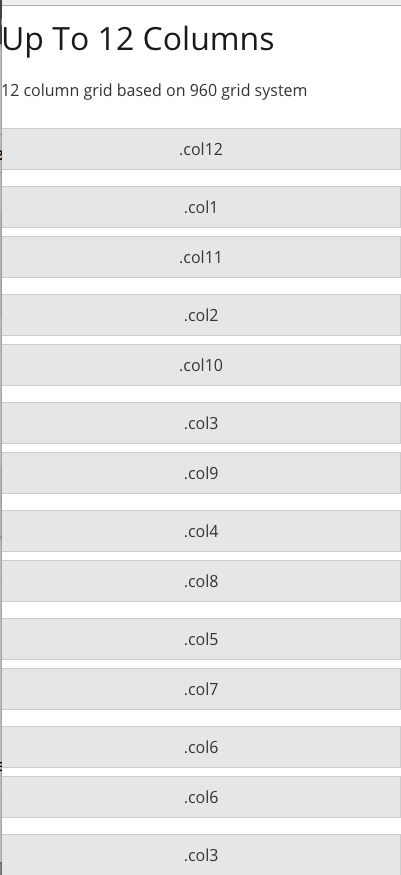
\includegraphics[scale=0.4]{images/collapsed}
\caption{Mobile View of Columns}
  \label{fig:collapsed}
\end{figure}

\newpage
\centering
\begin{figure}[ht]
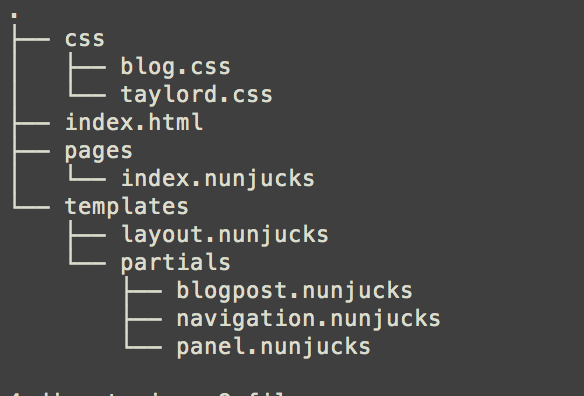
\includegraphics[scale=0.5]{images/fileStructure}
\caption{Nunjucks File Structure}
  \label{fig:structure}
\end{figure}

\begin{figure}[ht]
\centering
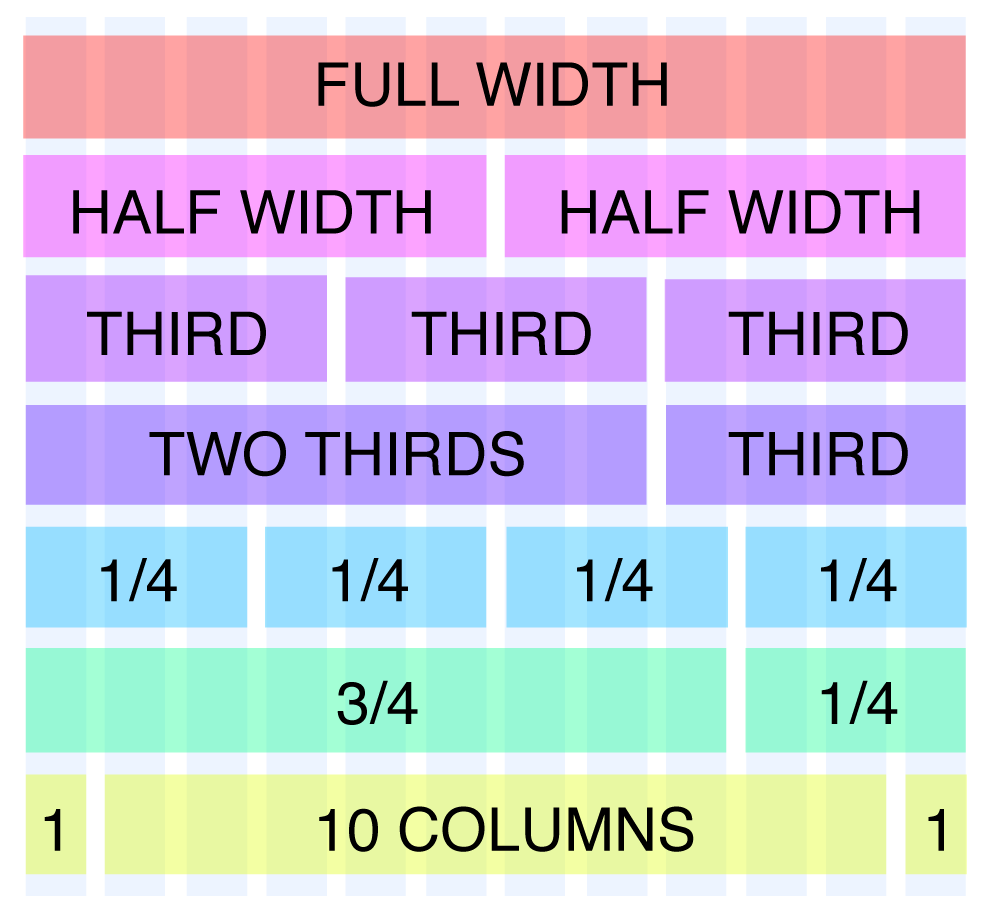
\includegraphics[scale=0.2]{images/960-12-col-grid}
\caption{12 Grid Layout with the 960 Grid}
  \label{fig:grid}
\end{figure}

\begin{figure}[ht]
\centering
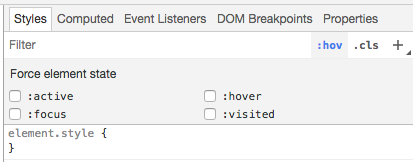
\includegraphics[scale=0.5]{images/tools}
\caption{Chrome Developer Tools}
  \label{fig:tools}
\end{figure}


\newpage
\begin{table}[!ht]
\centering
\caption{Framework features}
\label{features}
\begin{tabular}{llll}
 & Bootstrap & Foundation & Skeleton \\
Alerts & Yes & Yes & No \\
Accordion & Yes & Yes & No \\
Badges & No & Yes & No \\
Breadcrumbs & Yes & Yes & No \\
Buttons & Yes & Yes & Yes \\
Carousel & Yes & Yes & No \\
Dropdown & Yes & Yes & No \\
Forms & Yes & Yes & Yes \\
Form Validation & Yes & Yes & No \\
Grid & Yes & Yes & Yes \\
Icons & No & Yes & No \\
Labels & Yes & Yes & No \\
Lists & Yes & Yes & Yes \\
Media Object & Yes & Yes & Yes \\
Modals & Yes & Yes & No \\
Navigation & Yes & Yes & No \\
Pagination & Yes & Yes & No \\
Panels & Yes & Yes & No \\
Popovers & Yes & Yes & No \\
Print Styles & Yes & Yes & Yes \\
Progress Bar & Yes & Yes & No \\
Responsive Media & No & Yes & No \\
Right to Left & No & Yes & No \\
Scrollspy & Yes & Yes & No \\
Tables & Yes & Yes & Yes \\
Tabs & Yes & Yes & No \\
Thumbnails & Yes & Yes & No \\
Tooltips & Yes & Yes & No \\
Typeahead & No & No & No \\
Typography & Yes & Yes & Yes \\
Video Scaling & Yes & Yes & No
\end{tabular}
\end{table}

\begin{table}
\centering
\caption{Column Layout}
\label{column}
    \begin{tabular}{lll}
    Layout  & ~ & Number of Columns \\
    2 x 480 & ~ & 2 columns         \\
    3 x 320 & ~ & 3 columns         \\
    4 x 240 & ~ & 4 columns         \\
    5 x 192 & ~ & 5 columns         \\
    6 x 160 & ~ & 6 columns         \\
    8 x 120 & ~ & 8 columns         \\
    10 x 96 & ~ & 10 columns        \\
    12 x 80 & ~ & 12 columns        \\
    16 x 60 & ~ & 16 columns        \\
    20 x 48 & ~ & 20 columns        \\
    24 x 50 & ~ & 24 columns        \\
    30 x 32 & ~ & 30 columns        \\
    \end{tabular}
\end{table}

%

%
%%%%%%%%%%%%%%%%%%%%%%%%%%%%%%%%%%%%%%%%%%%%%%%%%%%%%%%%%%%%%%%%%%%%%%%%%%%%%%%%%%%%%

%
\bibliographystyle{plainnat}
\bibliography{bibliography/bibtex}
\addcontentsline{toc}{chapter}{Bibliography}
%

\end{document}


